\documentclass[11pt, oneside]{article}   	% use "amsart" instead of "article" for AMSLaTeX format


%\usepackage{draftwatermark}
% \SetWatermarkText{Confidential}
% \SetWatermarkScale{5}
% \SetWatermarkLightness {0.85} 
% \SetWatermarkColor[rgb]{0.7,0,0}


\usepackage{geometry}                		% See geometry.pdf to learn the layout options. There are lots.
\geometry{letterpaper}                   		% ... or a4paper or a5paper or ... 
%\geometry{landscape}                		% Activate for for rotated page geometry
%\usepackage[parfill]{parskip}    		% Activate to begin paragraphs with an empty line rather than an indent
\usepackage{graphicx}				% Use pdf, png, jpg, or eps� with pdflatex; use eps in DVI mode
								% TeX will automatically convert eps --> pdf in pdflatex		
\usepackage{amssymb}
\usepackage{hyperref}
\usepackage{url}
\usepackage{authblk}
\usepackage{amsmath}
\usepackage{graphicx}
\usepackage{fixltx2e}
\usepackage{hyperref}
\usepackage{alltt}
\usepackage{color}


\title{Notes on Sequence to Sequence Learning with Neural Networks}

\author{David Meyer \\ dmm@brocade.com}

% \date{}							% Activate to display a given date or no date


\begin{document}
\maketitle
\begin{abstract}

\end{abstract}
\section{Introduction} 

The purpose of this document is to (i). make a few notes on \cite{SEQ2SEQ} and (ii). fill in some of the gaps in the math that underlies the paper. 

\section{Logistic Regression}
\label{sec:logistic_regression}

Since Sequence to Sequence Learning~\cite{SEQ2SEQ} uses two LSTMs, one for the input sequence and one for the output sequence which follow the formulation given in Graves~\cite{GRAVES2013}. Figure~\ref{fig:prediction_architecture} shows the structure of the prediction architecture used there. More detail on the architecture of LSTM cells is shown in Figure~\ref{fig:lstm_cell} (note that this design uses the so-called "peephole connections").

\begin{figure}
\begin{center}
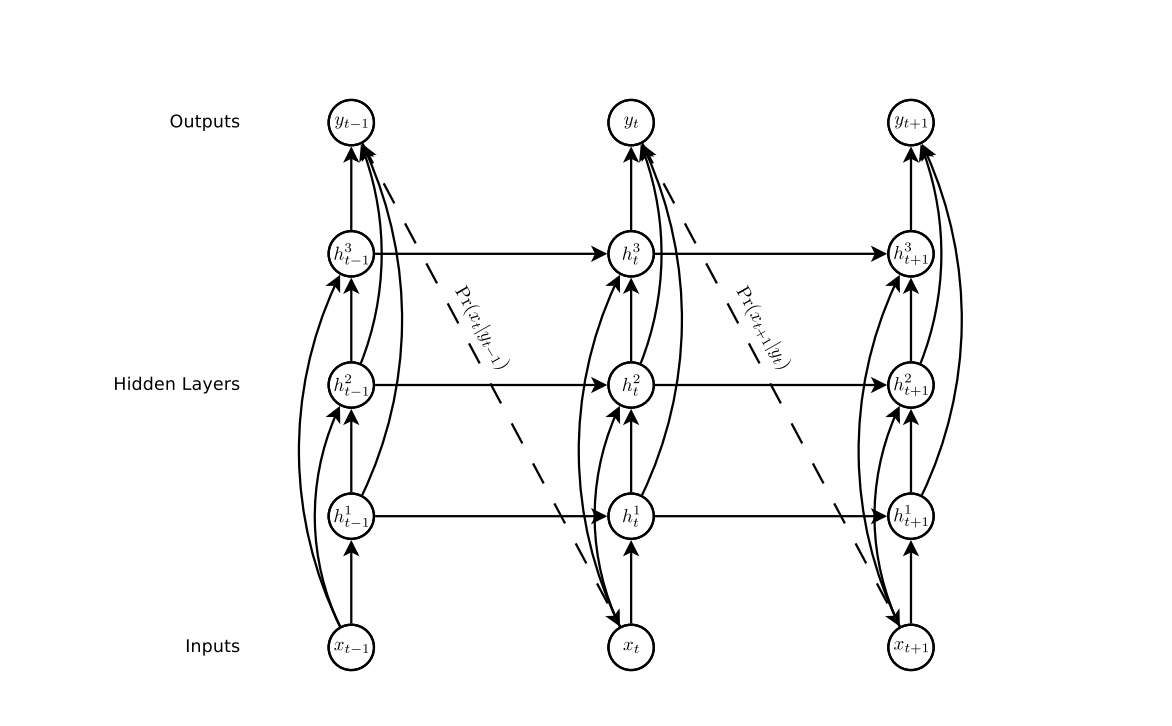
\includegraphics [width=10cm, height=7cm] {images/prediction_architecture.png}
\caption {Deep RNN Prediction Architecture from Graves \cite{GRAVES2013} %
    \label{fig:prediction_architecture}}
\end{center}
\end{figure}
\label{fig:prediction_architecture}


Graves~\cite{GRAVES2013} models sequences as a multinomial distribution which can be naturally parameterized by a softmax function at the output layer. That is, if there are $K$ text classes in total and class $k$ is read at time $t$, then $x_t$ is a $K$ length vector which is one-hot encoded (all of its entries are zero except for the $k^{th}$ entry which is one). Hence $Pr(x_{t+1} = k \mid y_t)$ is a multinomial distribution:

\begin{equation}
Pr(x_{t+1} = k \mid y_t) = y_{t}^{k} = 
\frac{e^{\hat{y}_{t}^{k}}}
{\sum\limits_{k^{\prime} = 1}^{K}e^{\hat{y}_{k\prime}^{k}}}
\end{equation}

\begin{figure}
\begin{center}
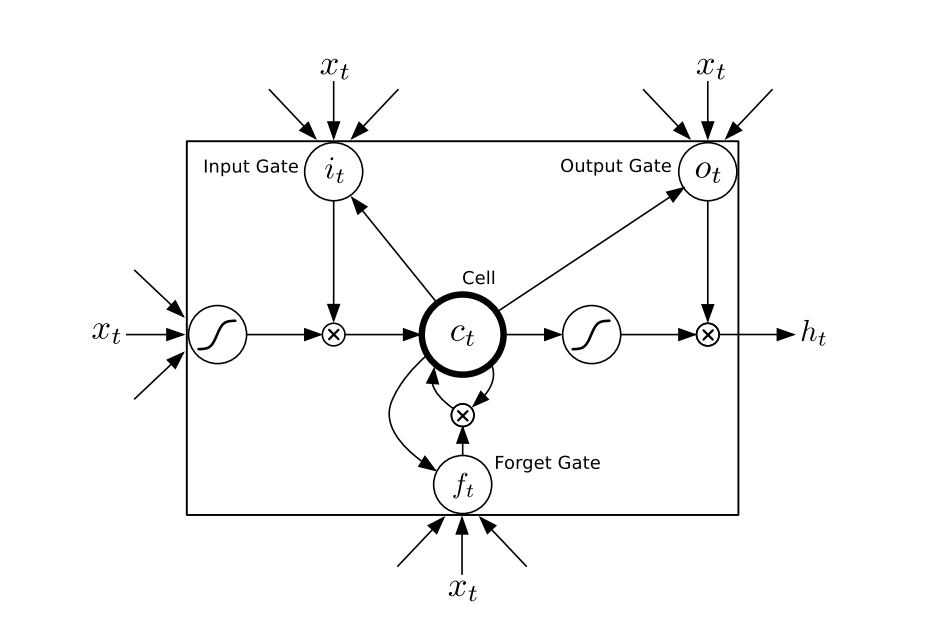
\includegraphics [width=10cm, height=7cm] {images/lstm_cell.png}
\caption {Long Short-Term Memory Cell %
    \label{fig:lstm_cell}}
\end{center}
\end{figure}

\subsection{LSTM Activations}

\begin{flalign}
i_t &= \sigma(W_{xi}x_t + W_{hi}h_{t-1} + W_{ci}c_{t-1} + b_i) \\
f_t & = \sigma(W_{xf}x_t + W_{hf}h_{t-1} + W_{cf}c_{t-1} + b_f) \\
c_t & = f_{t}c_{t-1} +  i_{t} \tanh(W_{xc}x_t + W_{hc}h_{t-1}  + b_c) \\
o_t & = \sigma(W_{xo}x_t + W_{ho}h_{t-1} + W_{co}c_{t} + b_o) \\
h_t & = o_{t} \tanh(c_t)
\end{flalign}



\bigskip
One way to understand the behavior of the multinomial distribution and its loss function $\mathcal{L}(x)$ is to see how we compute the required gradients for logistic regression. Recall the that \emph{logistic function} $\sigma(x)$ is defined as follows:

\bigskip
\begin{flalign}
\sigma(x) & = \frac{1}{1 + e^{-x}}
\end{flalign}

\bigskip

We are actually interested in the derivative of $\sigma(x)$ so that we can compute gradients for back propagation. Looking forward, note that the \emph{softmax} classifier, which is used in~\cite{SEQ2SEQ}, is defined as follows:

\begin{flalign}
p_j & = \frac{e^{o_j}}{\sum\limits_{k = 1}^{K}e^{o_k}}
\end{flalign}

\bigskip

When $i = j$ the derivative of softmax is similar to the derivative of the logistic function, which why its useful to look at the logistic function.

\bigskip

\subsection{Derivative of the Logistic Function}
\label{lr_regression}
Recall the \emph{chain rule} for derivatives is
\bigskip
\begin{equation}
\label{chain_rule.1}
\frac{d}{dx}\Big[f(g(x)\Big] = f^\prime(g(x))g^\prime(x))]
\end{equation}
\bigskip

Now, let the logistic function $\sigma(x) = \frac{1}{1 + e^{-x}}$. Then for purposes of the chain rule we define

\bigskip
\begin{flalign*}
g(x) & = 1 + e^{-x} \\
f(x) & = \frac{1}{x}
\end{flalign*}

\bigskip
so that $\sigma(x) = f(g(x)) = \frac{1}{1 + e^{-x}}$.  Taking the derivatives of $g$ and $f$ we get
\bigskip

\begin{flalign}
g^{\prime}(x) &  = e^{-x} \\
f^{\prime}(g(x)) &  = (1 + e^{-x})^{-2}
\end{flalign}

\bigskip
Given these definitions, we have:

\begin{flalign*}
& \frac{d \sigma(x)}{dx} = \frac{d}{dx} \Big [f(g(x))\Big]  = f^\prime(g(x)) g^\prime(x) \\
& = \frac{e^{-x}}{(1 + e^{-x})^2} \\
& = \frac{1 + e^{-z} -1}{(1 + e^{-z})^2} \\
& = \frac{1 + e^{-z}} {(1 + e^{-z})^2} - \left(\frac{1}{1 + e^{-z}}\right)^2 \\
& = \frac{1} {(1 + e^{-z})} - \left(\frac{1}{1 + e^{-z}}\right)^2 \\
& = \frac{1} {(1 + e^{-z})} \left(1 - \frac{1} {(1 + e^{-z})}\right) \\
& = \sigma(x) (1 - \sigma(x)) 
\end{flalign*}

\bigskip

This result is sometimes written as $\frac{dy_i}{dz_i}  = y_i (1 - y_i)$.


\section{Softmax}
\label{softmax}
The following describes the derivative of the softmax function. Recall that the softmax function is defined as follows:

\begin{flalign*}
p_j = \frac{e^{o_j}}{\sum\limits_{k = 1}^{K}e^{o_k}} \\
\end{flalign*}

When $i = j$, the softmax function derivative is similar to the derivative of the logistic function, namely:
\bigskip
\begin{equation}
\frac{\partial y_i}{\partial z_i} = y_i (1 - y_i)
 \end{equation}
 
 \bigskip
Since \cite{SEQ2SEQ} follows the notation and approach outlined in \cite{GRAVES2013}, it is useful to understand the derivation of the derivative of the loss function $\mathcal{L}(x)$ defined there. 
 \begin{equation}
 \label{likelihood.1}
 \mathcal{L}(x) = - \sum\limits_{t = 1}^{T} \log y_t^{x_t+1}
 \end{equation}
 
 For the purposes of the derivation, we'll use 
\bigskip
\begin{equation}
\label{likelihood.2}
\mathcal{L}(x) = - \sum\limits_{j} t_j \log y_i
\end{equation}
 
 Applying the chain rule gives us 
 \bigskip

 \begin{equation}
 \frac{\partial \mathcal{L}(x)}{\partial z_i} = - \frac{\partial \mathcal{L}(x)}{\partial y_i} \cdot \frac{\partial y_i}{\partial z_i} 
 \end{equation}
 
 \bigskip
Then the gradient of the loss function $\frac{\partial \mathcal{L}(x)}{\partial z_i}$ can be derived as follows: 
 
\begin{flalign*}
\frac{\partial \mathcal{L}(x)}{\partial z_i} & = - \frac{\partial \mathcal{L}}{\partial y_i} \left[\sum\limits_{j}^{}t_j \cdot \log y_i \right] (y_i \cdot (1 - y_i)) \\
& = - t_j \frac{\partial \mathcal{L}}{\partial y_i} \log y_i \cdot (y_i \cdot (1 - y_i)) \\
& = - t_j \frac{1}{y_i} \cdot (y_i \cdot (1 - y_i)) \\
& = - (t_j \cdot (1 - y_i)) \\
& = y_i - t_j
\end{flalign*}

\bigskip
Note that $\frac{\partial{y_i}}{\partial{z_i}}$ is replaced with $y_i  (1 - y_i)$ in the above (Section~\ref{lr_regression}).  Graves~\cite{GRAVES2013} uses an analogous derivation to get the following result:

\begin{equation}
\begin{split}
\mathcal{L}(x) = - \sum\limits_{t = 1}^{T} \log y_t^{x_t+1} \\
\Longrightarrow \frac{\partial{\mathcal{L}(x)}} {\partial{\hat{y}_t^k}} = y_{t}^{k} - \delta_{k, x_{t+1}}
\end{split}
\end{equation}

\section{Acknowledgements}

\newpage
% \cite{test}
\bibliographystyle{plain}
\bibliography{/Users/dmm/papers/bib/ml}
% \bibliography{/Users/dmm/papers/bib/rfc}


\end{document}  


% \begin{equation}
% KL(\rho\parallel\hat{\rho}) = \rho \log\frac{\rho}{\hat{\rho_{j}}} + (1 - \rho) \log \frac{1 - \rho}{1 - \hat{\rho_{j}}}
% \label{eqn:KL}
% \end{equation}

% \begin{equation}
% \begin{array}{cc}\text{minimize} \\ {W_{1}, W_{2}}\end{array}
% \sum\limits_{i = 1}^{m}
% (\parallel {W_{2}W_{1}^{T}x^{(i)} - x^{(i)}}\parallel_{2}^{2}
% + \lambda\sum\limits_{j = 1}^{k}\sqrt{\epsilon + H_{j}(W_{1}^{T}x^{(i)})^{2}})
% \label{eqn:google}
% \end{equation}
